\documentclass[a4paper]{article}

\usepackage{titlesec}
\usepackage{listings}
\usepackage{graphicx}
\usepackage{color}
\usepackage[margin=1.2in]{geometry}
\usepackage{algorithm}
\usepackage{algorithmic}
\usepackage{commath}
\usepackage{moreverb}
\usepackage{amssymb,amsmath}

\usepackage[colorlinks=true,
            allcolors=green]{hyperref}

\newcommand{\kora}{%
(\raisebox{0.5em}{\rotatebox{-45}{)}}$^{\circ}{\scriptscriptstyle\Box}^{\circ}$)\raisebox{0.5em}{\rotatebox{-45}{)}}\rotatebox{90}{)}\raisebox{0.2em}{\LARGE \_\hskip-.1em\textvisiblespace\hskip-.1em\_}
}

\title{Analysis of Lab\_\#2: Mix of (Abstract) Factory and Decorator Pattern}

\makeatletter
\renewcommand{\maketitle}{\bgroup\setlength{\parindent}{0pt}
    \begin{center}

        \textbf{\Large\@title} \\[12pt]


        \par\vspace{\baselineskip}
    \end{center}

\egroup}
\makeatother

\titleformat{\section}
{\large\bfseries}
{\thesection}
{0.5em}
{}

\lstset{
    frame=single
}

\begin{document}
\maketitle


\section{Analysis of Lab 2}%
\label{sec:analysis_of_lab_2}

In this lab, we are required to solve some real-world problems
by fusing patterns including \textit{Abstract Factory Pattern},
\textit{Factory Pattern} and \textit{Decorator Pattern}. The question
provides situations: ``vendors $\to$ stores $\to$ client'' and we
select \textbf{case 2} to complete.

First of all, we implement the vendors side with \textit{Decorator Pattern},
all of the components are capable of offering not only the price
of the computing blocks itself, but also the previous (former, inside)
prices of products inside the wrapped, each of which also performs
as a certain type of blocks say \texttt{CPU} and so on. Second, we
build the selling store with an ability of dynamic components
providing alteration, undertaking tasks of constructing the blocks
from piece to piece, to a more concrete and entire object computer,
which also maintains an interface of inspection, to the later supervision
side. Then comes the department ensuring the quality of the products,
which counts the components types to three, any of which belows three
will be definitely labeled as ``disqualified''. Note the report
is illustrated based on conventions
\footnote{\underline{package}, \texttt{class}, \textbf{file}, \textsl{method}, \textit{pattern}}
in previous one.

\section{Patterns}%
\label{sec:patterns}

\begin{figure}[h]
    \centering
    \includegraphics[width=0.6\textwidth]{do.png}
    \caption{Patterns coupling}
    \label{fig:pattern_coupling}
\end{figure}

We strive to illustrate the patterns we harboured in this project in this section\ref{sec:patterns}.
We define the computing blocks to be the decorator, each of which is
also able to wrap the \texttt{ComputerBase} (actually we do need a base representing the labor of
the company). Then we pick the vendors \texttt{Intel} and \texttt{Samsung}
out to be the \textit{Abstract Factory} for they should behave like
exposing the interface of producing three types of computing blocks
(if a factory provides more than one product, then it is an abstract factory).
Then comes the upper-level abstraction of the task, the store (also known as \texttt{LaptopCompany} and \texttt{PCCompany}),
which is implemented in \texttt{Factory Pattern} for they should
offer behaviour resembling providing the client with only ONE product.

\section{Non Pattern Things}%
\label{sec:non_pattern_things}

Patterns are straightforward and easy to understand
as illustrated in figure\ref{fig:pattern_coupling}, still,
addressing consideration that the task is presented with some behaviour we can hardly
extract a pattern, we carry out abstractions as order, order-decoding
and decoration-unfolding. Thus we'll cover the thoughts of our design and
tricks of implementation.

\subsection{Order}%
\label{sub:order}

For a set of requirements of the client, \textsl{ArrayList$<$Pair$<$String, Pair$<$String, String$>>>$}
is utilized for growth-allowed list with nested pair like ``Intel, CPU, i7''.
The abstraction is so real that the client should make any order with ease.


But things have become a little weird for the programmer to
make these requirements done correctly, aiming at solving which,
the \texttt{Company} takes responsibilities of the order decoding.

\subsection{Order Decoding}%
\label{sub:order_decoding}

On the stage of receiving requisites of the customers,
the company first,
between the lines of code,
loops through each of the nested pair
and send it to the \textsl{produce()} method,
each of which will be dispatched to certain factory with
a previous reference of decorator to be the parameter of
current constructor, so as to hold a \textsl{ArrayList$<$String$>$}
representing chaining of prices. This behaviour is
quite simple, for in real-world, the seller would do the same
as redirections of building blocks to the vendors of components.

\begin{figure}[h]
    \centering
    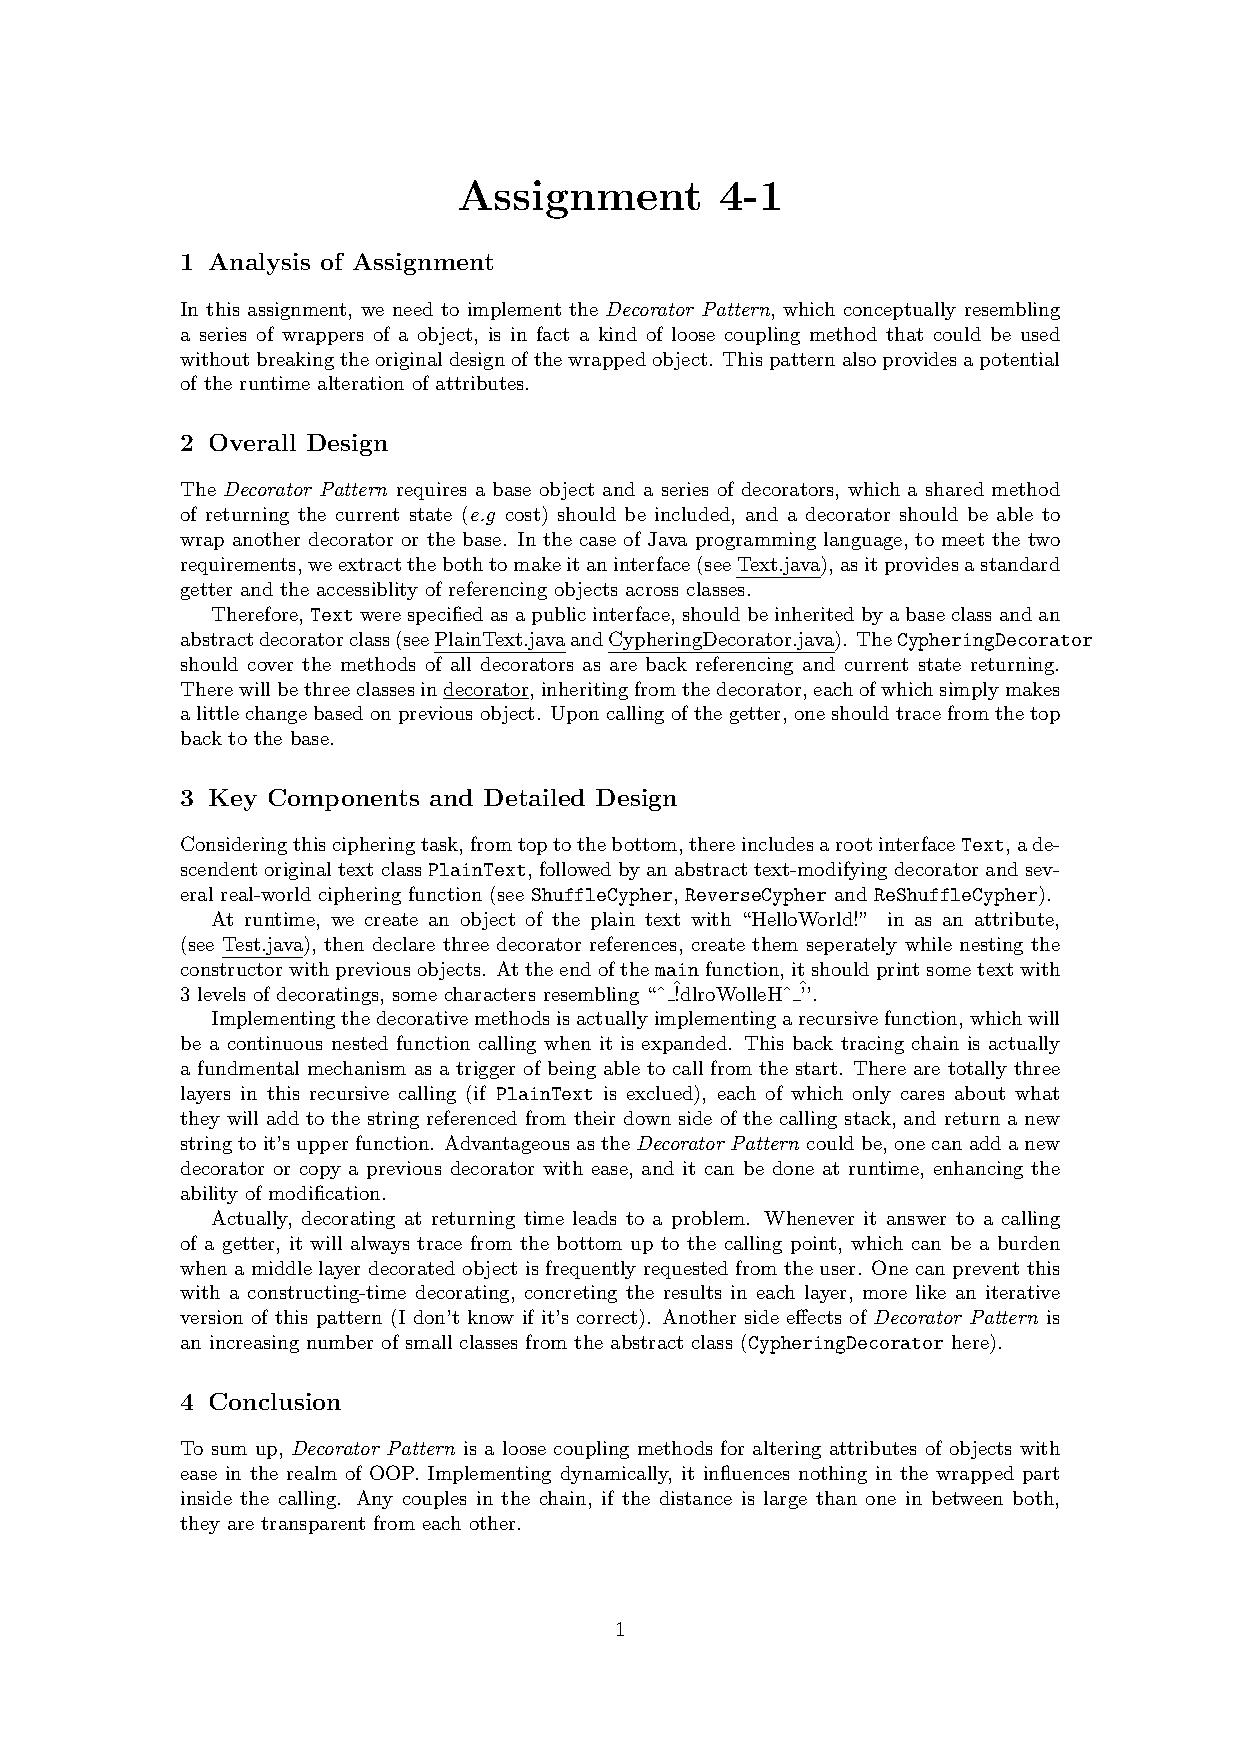
\includegraphics[width=0.6\textwidth]{decorator.png}
    \caption{Decorator as wrapped object}
    \label{fig:decorator}
\end{figure}

Storing as a wrapped object, any of the abstraction can hardly
know the amount and types the computer consisted of, as it leads
to our tricks: \textsl{instanceof} and Java reflection.

For each of the computing blocks, as we define ``price'' to
represent as a recursive alteration of decorator,
though we can modify the decorator chain to be a more
complex object, still we carry out the feature ``reflection''
of Java to extract the class name of the object as \textsl{obj.getClass().getSimpleName()}
to obtain the name of the components as it's more convenient.

\subsection{Decoration Unfolding}%
\label{sub:decoration_unfolding}

Obviously as displayed in figure\ref{fig:decorator},
one can hardly identify all types of the these computing blocks from only
the outest decorator,
expecting to overcome this, we propose a method using recursive
methods and Java \textsl{instanceof} features. To be specific,
every time the company is in need of a storage of the
components as \textsl{ArrayList$<$Product, Integer$>$},
it will not only ask the outer decorator to return an addition of
his price and the former prices in \textsl{ArrayList$<$String$>$} but also for
the type of these components through condition branches with \textsl{instanceof} as all computing blocks
implement the types (\texttt{CPU}, \texttt{RAM} and \texttt{Board} respectively)
for types recognition.
The algorithm is presented in this chart\ref{algorithm}.


\begin{algorithm}\label{algorithm}
\caption{Chain of Recursive Calling}
\begin{algorithmic}[1]
    \REQUIRE $Interface$ $CPU$, $RAM$, $Board$ in $Types$ and a $reference$ $D$
    \REQUIRE Global counter as cnt[3] for three types
    \STATE initialize a reference $P$ for previous $D$
    \IF{$P$ is \NOT $NULL$ \AND is \textsl{instanceof} $Types$}
        \STATE jumps to $1$ with $P$ as $D_{new}$
    \ENDIF
    \IF{$D$ is in $Types$}
    \STATE cnt[$D$] add 1
    \ENDIF
    \STATE done
\end{algorithmic}
\end{algorithm}

\section{Conclusion}%
\label{sec:conclusion}

In this lab, we finished the task with patterns: \textit{Abstract Factory}, \textit{Factory}
and \textit{Decorator}, to construct the business logic ``client $\to$ company $\to$ vendor'' in figure\ref{fig:pattern_coupling},
for a loose coupling design. We first addressed that three of the design patterns\ref{sec:patterns} we've managed
could be taken advantages of, then we mentioned that there are
utilities patterns can hardly cover so as being taken place of
by abstract behaviour as illustrated in section\ref{sec:non_pattern_things},
in which (\ref{sub:order_decoding} and \ref{sub:decoration_unfolding})
we've solved utilizing the features of Java language, achieving demands
of \textbf{case 2}. Hopefully we've illustrated this task and
our solution clearly and accurately.

\section{Appendix}%
\label{sec:appendix}

We want to add more detailed illustrations of our work here
\footnote{All UML diagrams are automatically generated by ObjectAid at \url{https://objectaid.com/home}}.

\subsection{Product}%
\label{sub:product}

As there are two vendors: \texttt{Samsung} and \texttt{Intel} company,
each of which is capable of providing the sellers (\texttt{LaptopCompany} and
\texttt{PCCompany}) three sorts computing blocks \texttt{CPU}, \texttt{RAM}
and \texttt{Mainboard}, each of which is divided into two types like
``large'' and ``tiny'', totally $2 \times 3 \times 2 = 12$ blocks, among
which we define decorators inside the \textsl{price()} to return the price, inside
of which then we save a temporary reference and ask the decorated to return his price.

\begin{figure}[h]
    \centering
    \includegraphics[width=1.0\textwidth]{UMLL2Product.jpg}
    \caption{Product, the decorators}
    \label{fig:product}
\end{figure}

\subsection{Company}%
\label{sub:company}

\begin{figure}[h]
    \centering
    \includegraphics[width=1.0\textwidth]{UMLL2Company.jpg}
    \caption{Company, the factory and abstract factory}
    \label{fig:company}
\end{figure}

In this section\ref{sub:company}, we implements the \textit{Factory Pattern},
as the actually store (connect directly with the client \textsl{main()})
contain a series of actions of building a computer thing. They adapt themselves
with a dynamic setter of abstract factory to deliver the customers
components-blended products according to the requirement.

\textit{Abstract Factory} is also included in this UML diagram,
they provide brand-set computing components with multiple interface
aiming at various types.


\subsection{Computer}%
\label{sub:computer}

This chart\ref{fig:computer} illustrates the procedure of producing
a computer (\texttt{Laptop} and \texttt{PC}) clearly and accurately.
During the period of building, the company asks the the top-level decorated
one for a list of components to constructing the computer, printing the
price for each blocks respectively. Passing the wrapped object to
\underline{SupervisionDepartment.java}, the client receives a laptop
or PC with an unique \textsl{UUID} and a boolean value representing
a qualification of itself.

\begin{figure}[h]
    \centering
    \includegraphics[width=1.0\textwidth]{UMLL2Computer.jpg}
    \caption{Computer}
    \label{fig:computer}
\end{figure}

\newpage

\subsection{output}%
\label{sub:output}

\begin{lstlisting}
15$ for base
25$ for SamsungCPUI7
12$ for IntelMainboardTiny
10$ for IntelMainboardLarge
35$ for SamsungRAM32G
20$ for IntelRAM16G
I'm a PC, and is a qualified PC
15$ for base
25$ for SamsungCPUI7
35$ for SamsungRAM32G
35$ for SamsungRAM32G
I'm a PC, and is not a qualified PC
20$ for base
30$ for IntelCPUI7
35$ for IntelCPUI9
35$ for SamsungRAM32G
35$ for SamsungRAM32G
12$ for SamsungMainboardTiny
I'm a Laptop, and is a qualified Laptop
\end{lstlisting}

\section{Additional Discussions}%
\label{sec:additional_discussions}

In this section, we want to discuss the differences among several patterns
associating with thoughts of wrapping an object.

\subsection{Decorator Pattern}%
\label{sub:decorator_pattern}

Conceptually a \textit{Decorator Pattern} is a pattern that
helps the building the attachment of additional behaviour or
responsibilities of an object dynamically without changing
the wrapped object inside the decorators.

In the realm of coding, the decorators and the base object share
a same interface that incurs a chain of calling of the desired
attributes. First we create a base object, then wrap (or decorate) it
with a optional decorator in the manner of composing a
reference to the inside object at constructing time. And we do that again and again
until the object is finished. Every time we want an attribute,
we ask the most outside layer to return an added attribute of the one just
inside of which is the closest to the wrapper outer layer.

On implementing this pattern, one should give consideration to
detailed syntax and features in the language he was planning
to use, resembling compositions and recursive matters. For instance
in \textbf{Java}, \texttt{protected} reference of the wrapped object
and the endpoint of recursive calls of the chain of the dynamical attributes
should be contained.

\subsection{Façade Pattern}%
\label{sub:facade_pattern}

\textit{Façade Pattern} is the easiest pattern among which we've learned. Just implement
a wrapper of a set of methods to make it be called only once once which were collected in
a single function, same effect as they were called separately.

Note that advanced data structure could be included in this pattern,
for each of the client which reacts variously, like tree or graph, is a
traversal of the operation set.

\subsection{Adapter Pattern}%
\label{sub:adapter_pattern}

Basically an \textit{Adapter Pattern} is a means of converting
an interface of an implemented object to another methods
without altering the interface itself by offering methods
of the adaptee inside the interface, appearing to be a fake cover
cause no one knows what is going on behind the scene.

So long as the adapter provides an implicit alteration of the exposed connection,
there exists two routes for building a \textit{Adapter Pattern}.
One is by carrying out the compositon of the adaptee's reference,
and the other one is to \texttt{extends} (implicitly refering by \texttt{this})
the adaptee to utilize the desired methods.

The \textit{Adapter Pattern} is quite straightforward and easy to understand. We can
manipulate any objects with any functions even some not belong to
the objects providing a mapping adapter from the covered to the original.

\end{document}
